\documentclass[11pt]{article}
\usepackage[margin=1in]{geometry}
\usepackage{graphicx}
\usepackage{multirow}
\usepackage{multicol}
\usepackage{setspace}

\setlength\parindent{0pt}
\usepackage{hyperref}
\usepackage{amssymb,amsthm,amsmath, fancyhdr}
\pagestyle{fancy}

\usepackage{lipsum}

\begin{document}
\chead{Math 121 - Limits involving infinity}
\begin{enumerate}
\item Evaluate each of these limits. Sketch a quick graph if it helps, and find the equation of the vertical asymptote, if there is one.
\begin{multicols}{2}
\begin{itemize}
    \item $\lim_{x\rightarrow 0^+} \frac{1}{x}$
    \item $\lim_{x\rightarrow 0^-} \frac{1}{x}$
    \item $\lim_{x\rightarrow 0} \frac{1}{x}$
    \item $\lim_{x\rightarrow 0^+} \frac{1}{x^2}$
    \item $\lim_{x\rightarrow 0^-} \frac{1}{x^2}$
    \item $\lim_{x\rightarrow 0} \frac{1}{x^2}$
\end{itemize}
\end{multicols}
\item Evaluate each of these limits. Refer to theorem 5 in the chapter 1.6 for a hint. Find the equations of the horizontal asymptotes, if there are any.
\begin{itemize}
    \item $\lim_{x \rightarrow \infty} \frac{2x-1}{3x+2}$
    \item $\lim_{x \rightarrow \infty} \frac{2x^2 + 5x -1}{5x^2 - 3x + 2}$
\end{itemize}
\item Using the graph below, find the equations of all horizontal and vertical asymptotes. Write each of them as a limit, either as $x \rightarrow \infty$, $x \rightarrow -\infty$, or as $x$ approaches a finite number, but where the limit is either $\infty $ or $-\infty$.\\
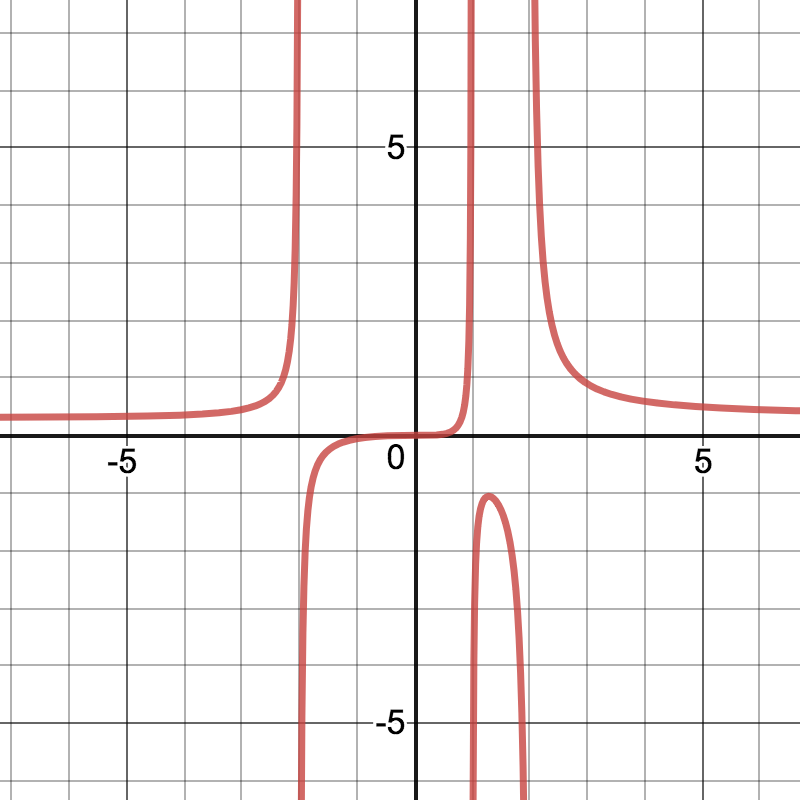
\includegraphics[width=0.7\textwidth]{Asymptotes.png}
\item In the theory of relativity, the mass of a particle with velocity $v$ is  
$$m = \frac{m_0}{\sqrt{1 - \frac{v^2}{c^2}}}.$$
What happens as $v \rightarrow c^-$?
\end{enumerate}
\end{document}